\section{Trigger Test of the Trailing Lepton}

In dilepton channel, at least one of leading and trailing lepton is 
required to pass the single lepton trigger.
In $e\mu$ channel, electron is required to fire single electron trigger and $p^T_e>p^T_\mu$.
In $\mu e$ channel, muon is required to fire single muon trigger and $p^T_\mu>p^T_e$.


Figure~\ref{fig:triggerTest} shows the trailing lepton \pt in the $\mu\mu$, $ee$, $\mu e$, $e\mu$ channel.
Events are split based on the trigger test of the leading and trailing lepton, which has four possible
scenarios, both pass (blue), only leading pass (origin), only trailing pass (green), both fail (red).
But the case of both fail should not appear due the event selection requirement. The scenario needs
attention is only the trailing lepton triggering the event. Since the shape analysis template fits the
trailing lepton \pt in the dilepton channel, it is good to know the contributions from such scenario and
decide whether extra treatment of trigger systematics is needed.


\begin{figure}[h!]
  \centering
  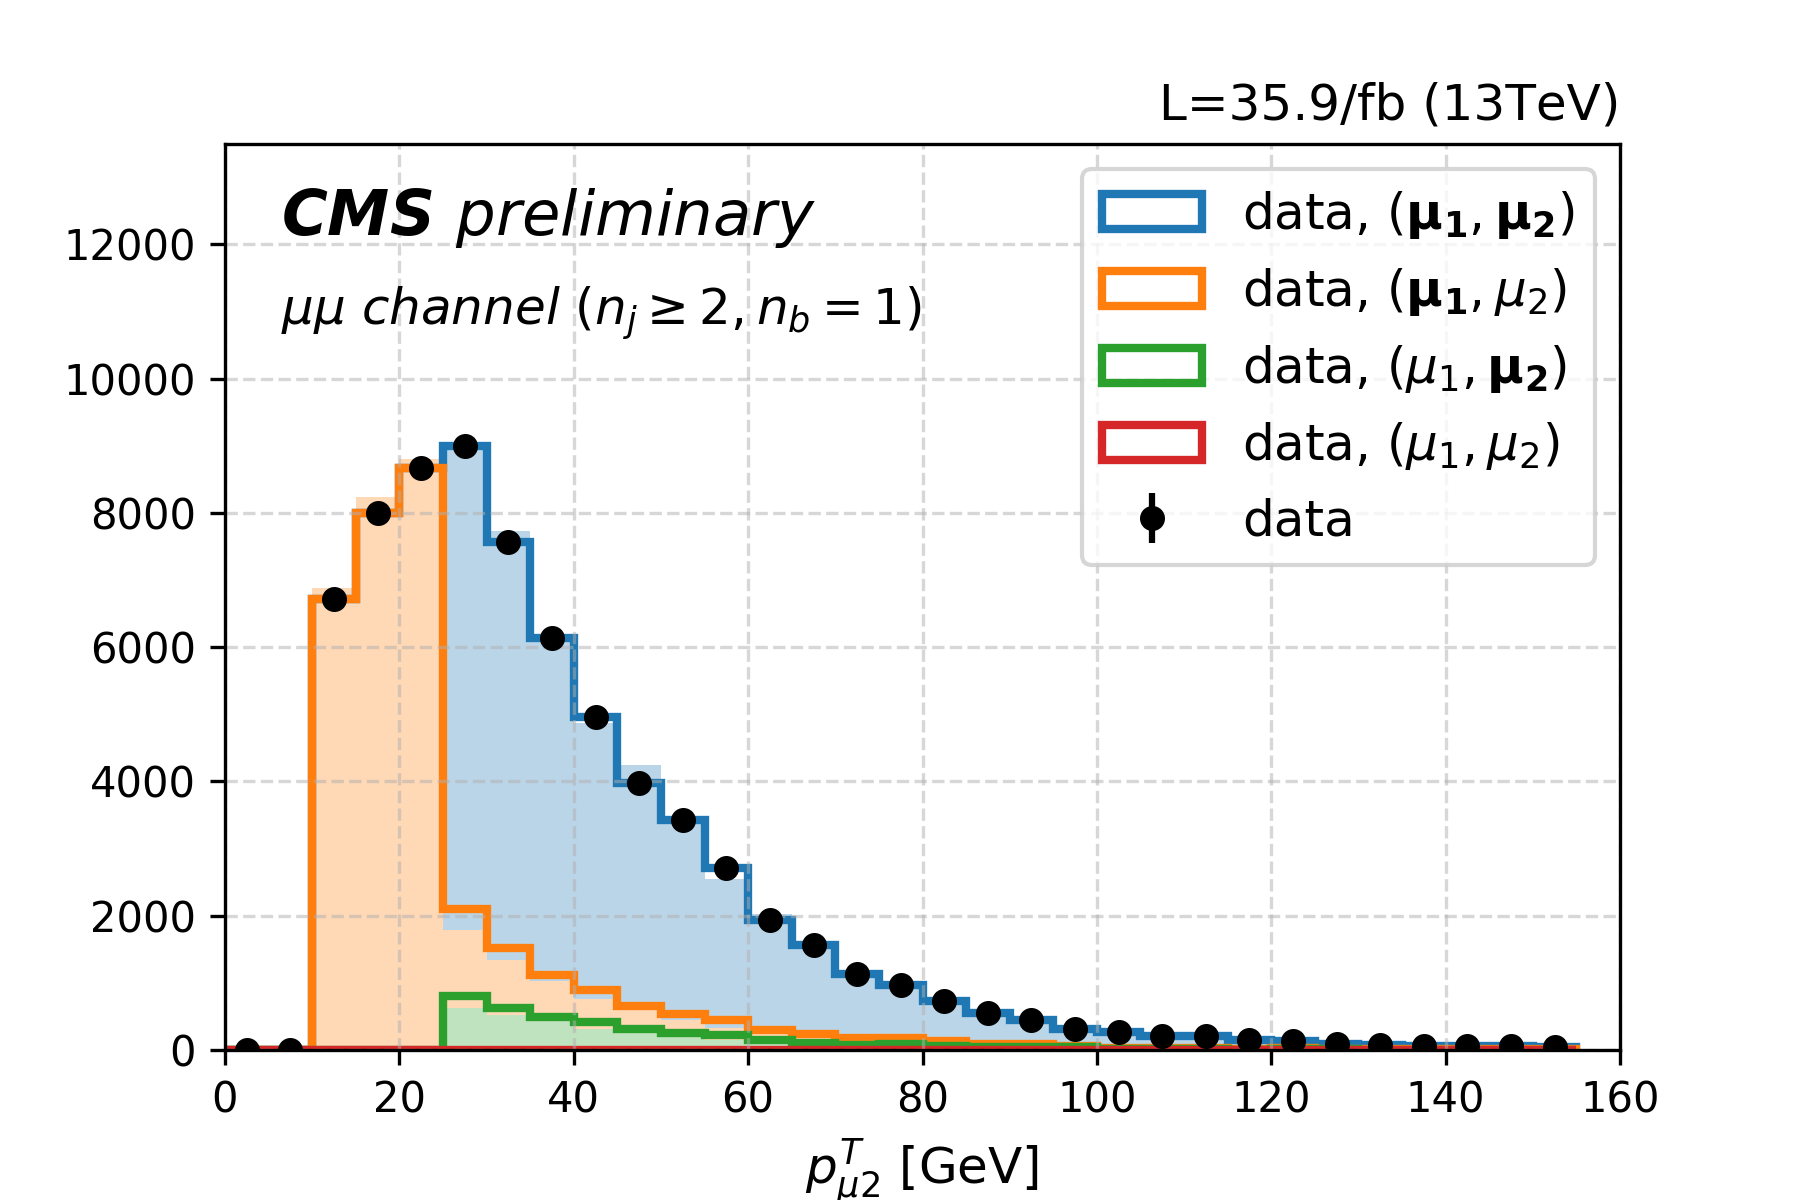
\includegraphics[width=0.49\textwidth]{chapters/Appendix/sectionTriggerTest/figures/trgLep_mumu.png}
  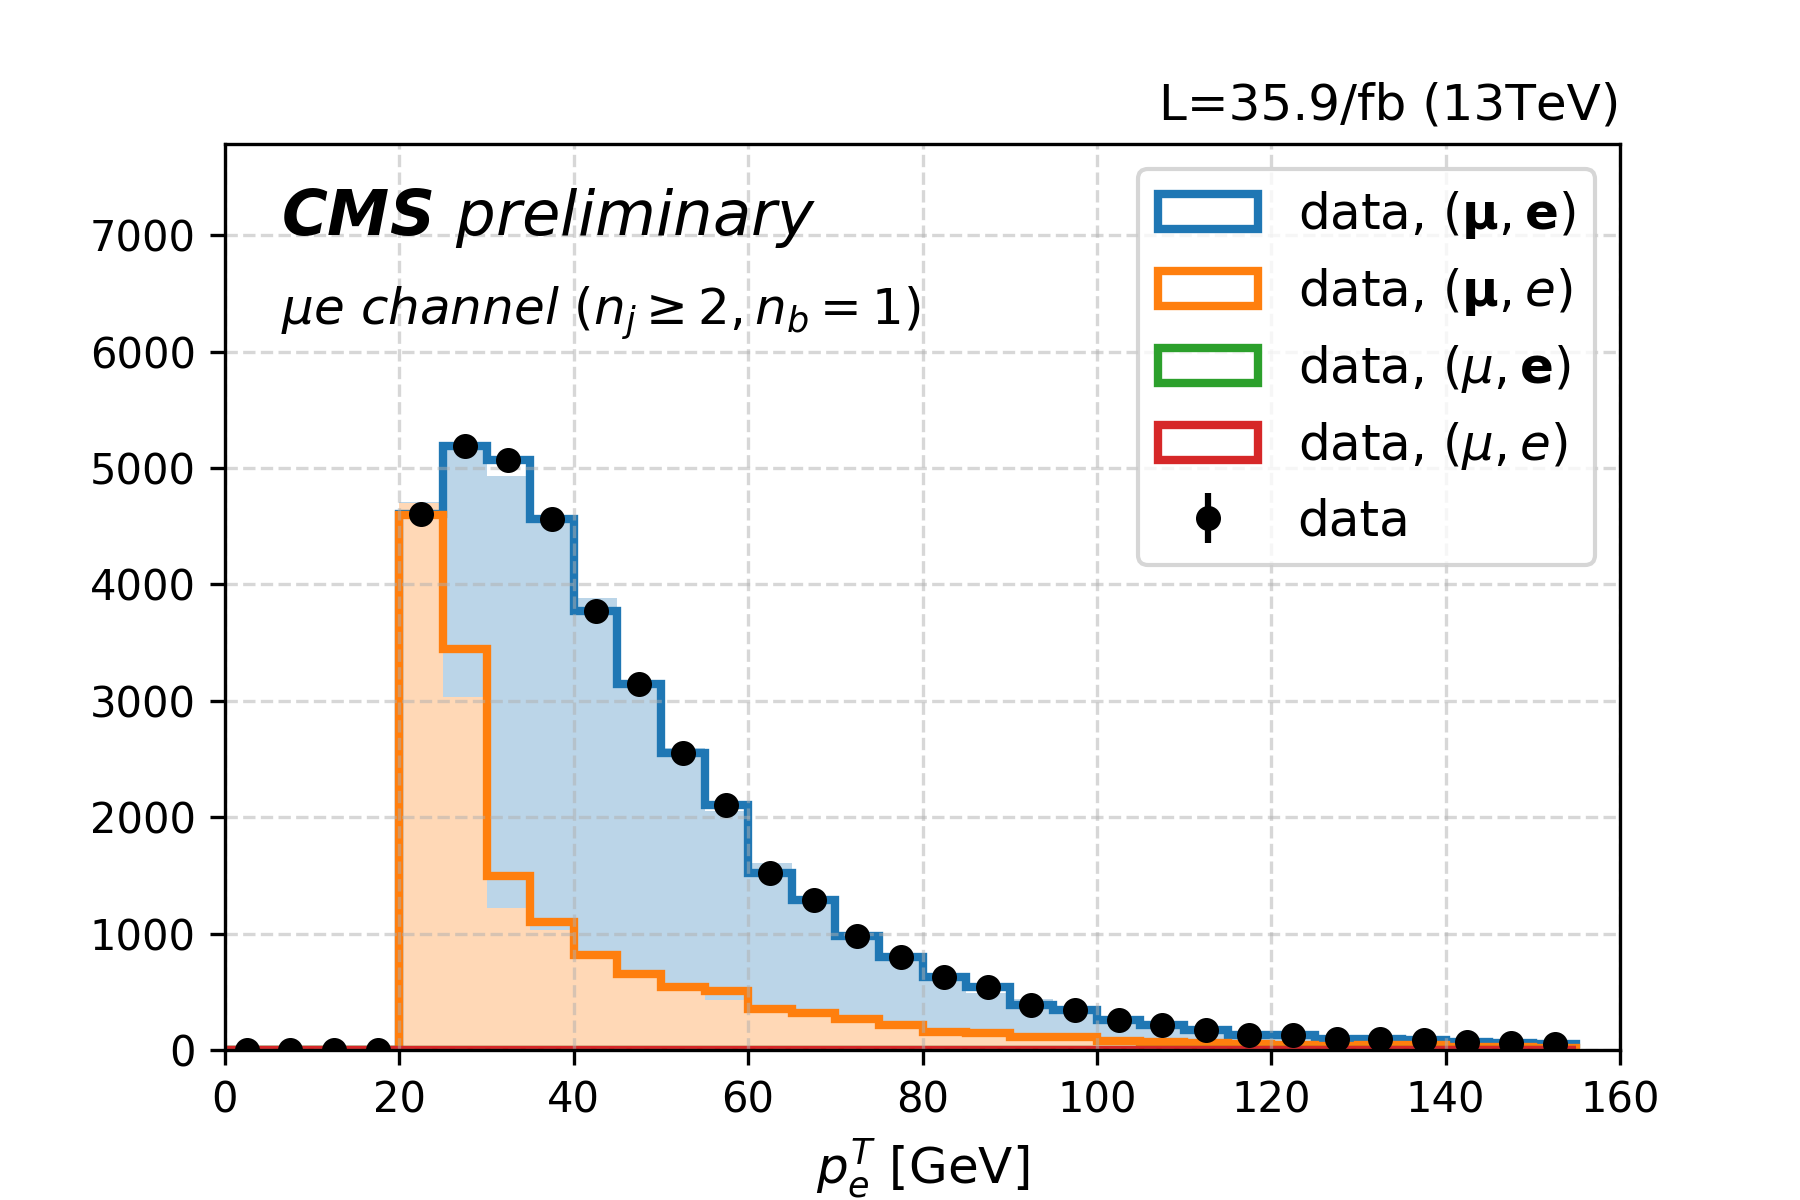
\includegraphics[width=0.49\textwidth]{chapters/Appendix/sectionTriggerTest/figures/trgLep_emu.png}
  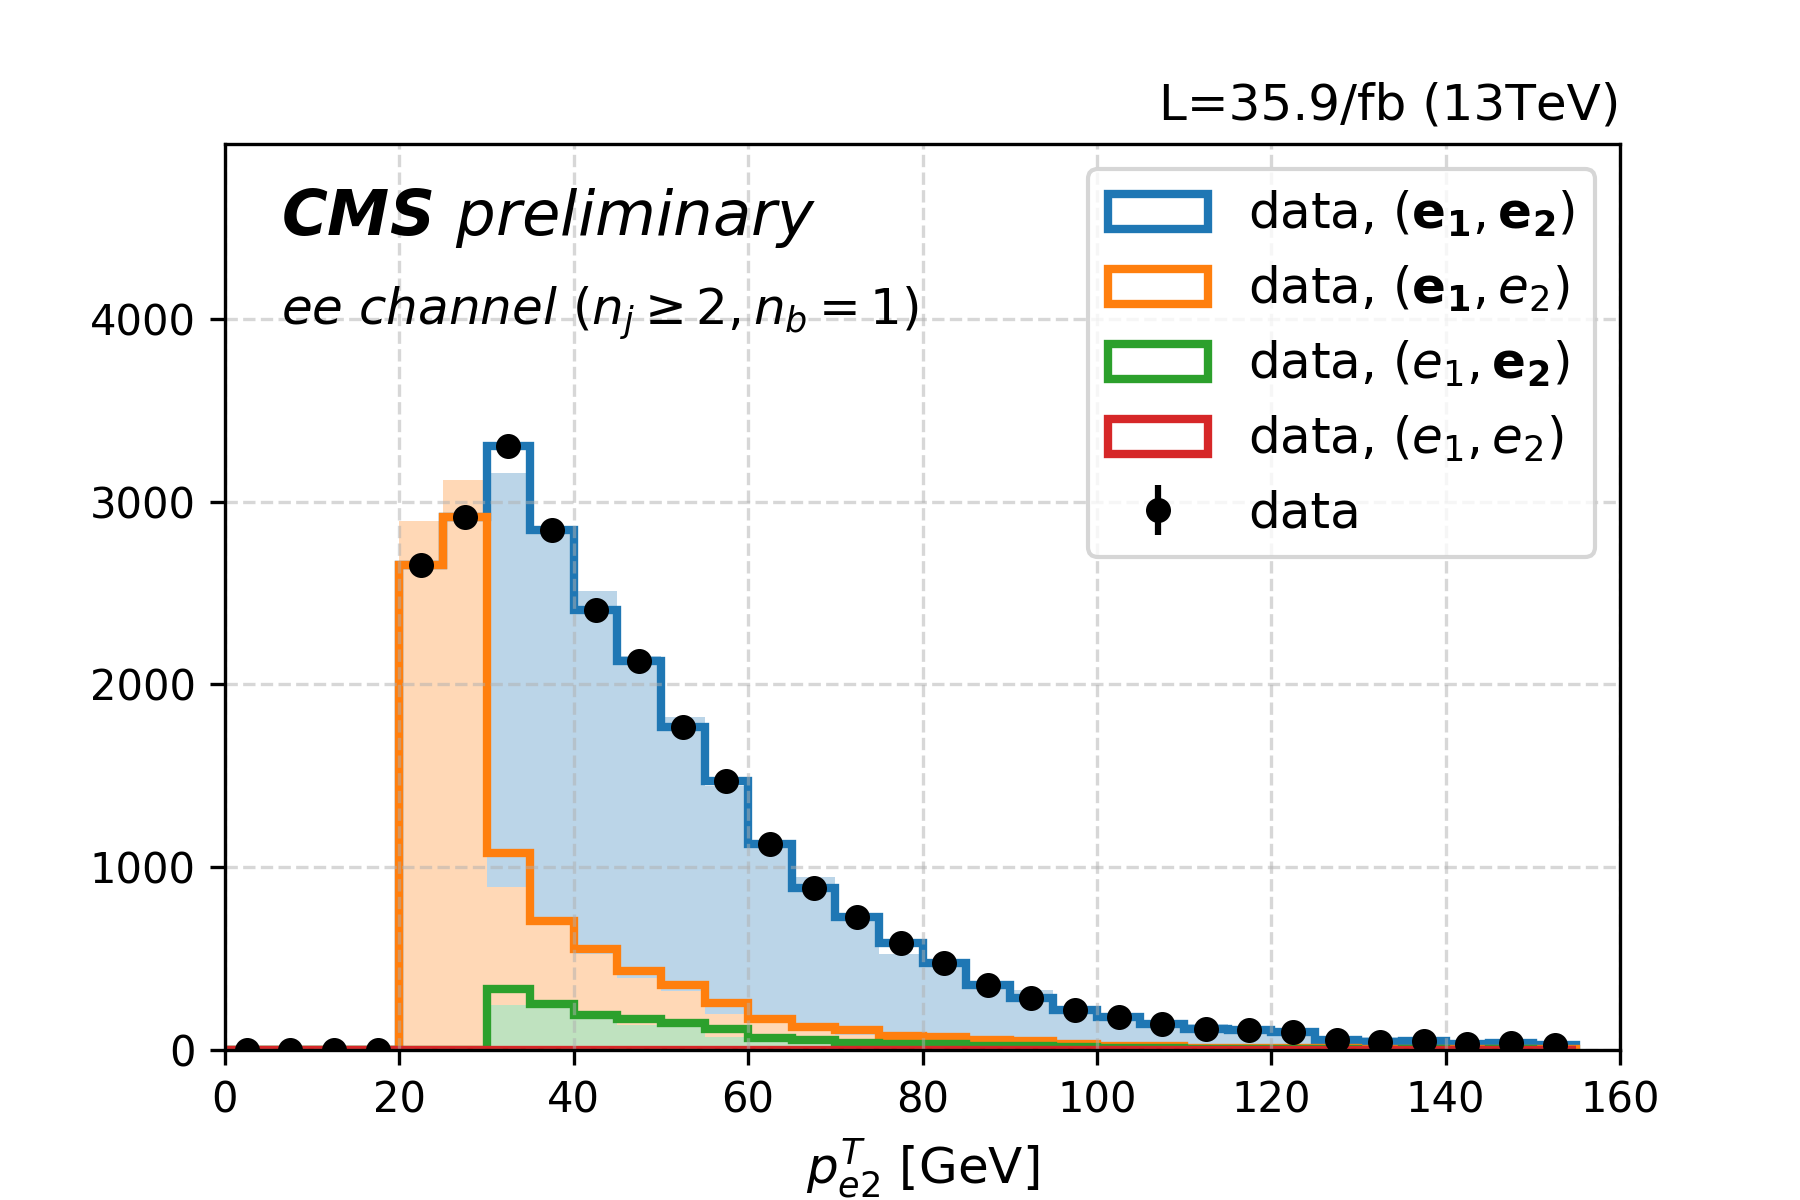
\includegraphics[width=0.49\textwidth]{chapters/Appendix/sectionTriggerTest/figures/trgLep_ee.png}
  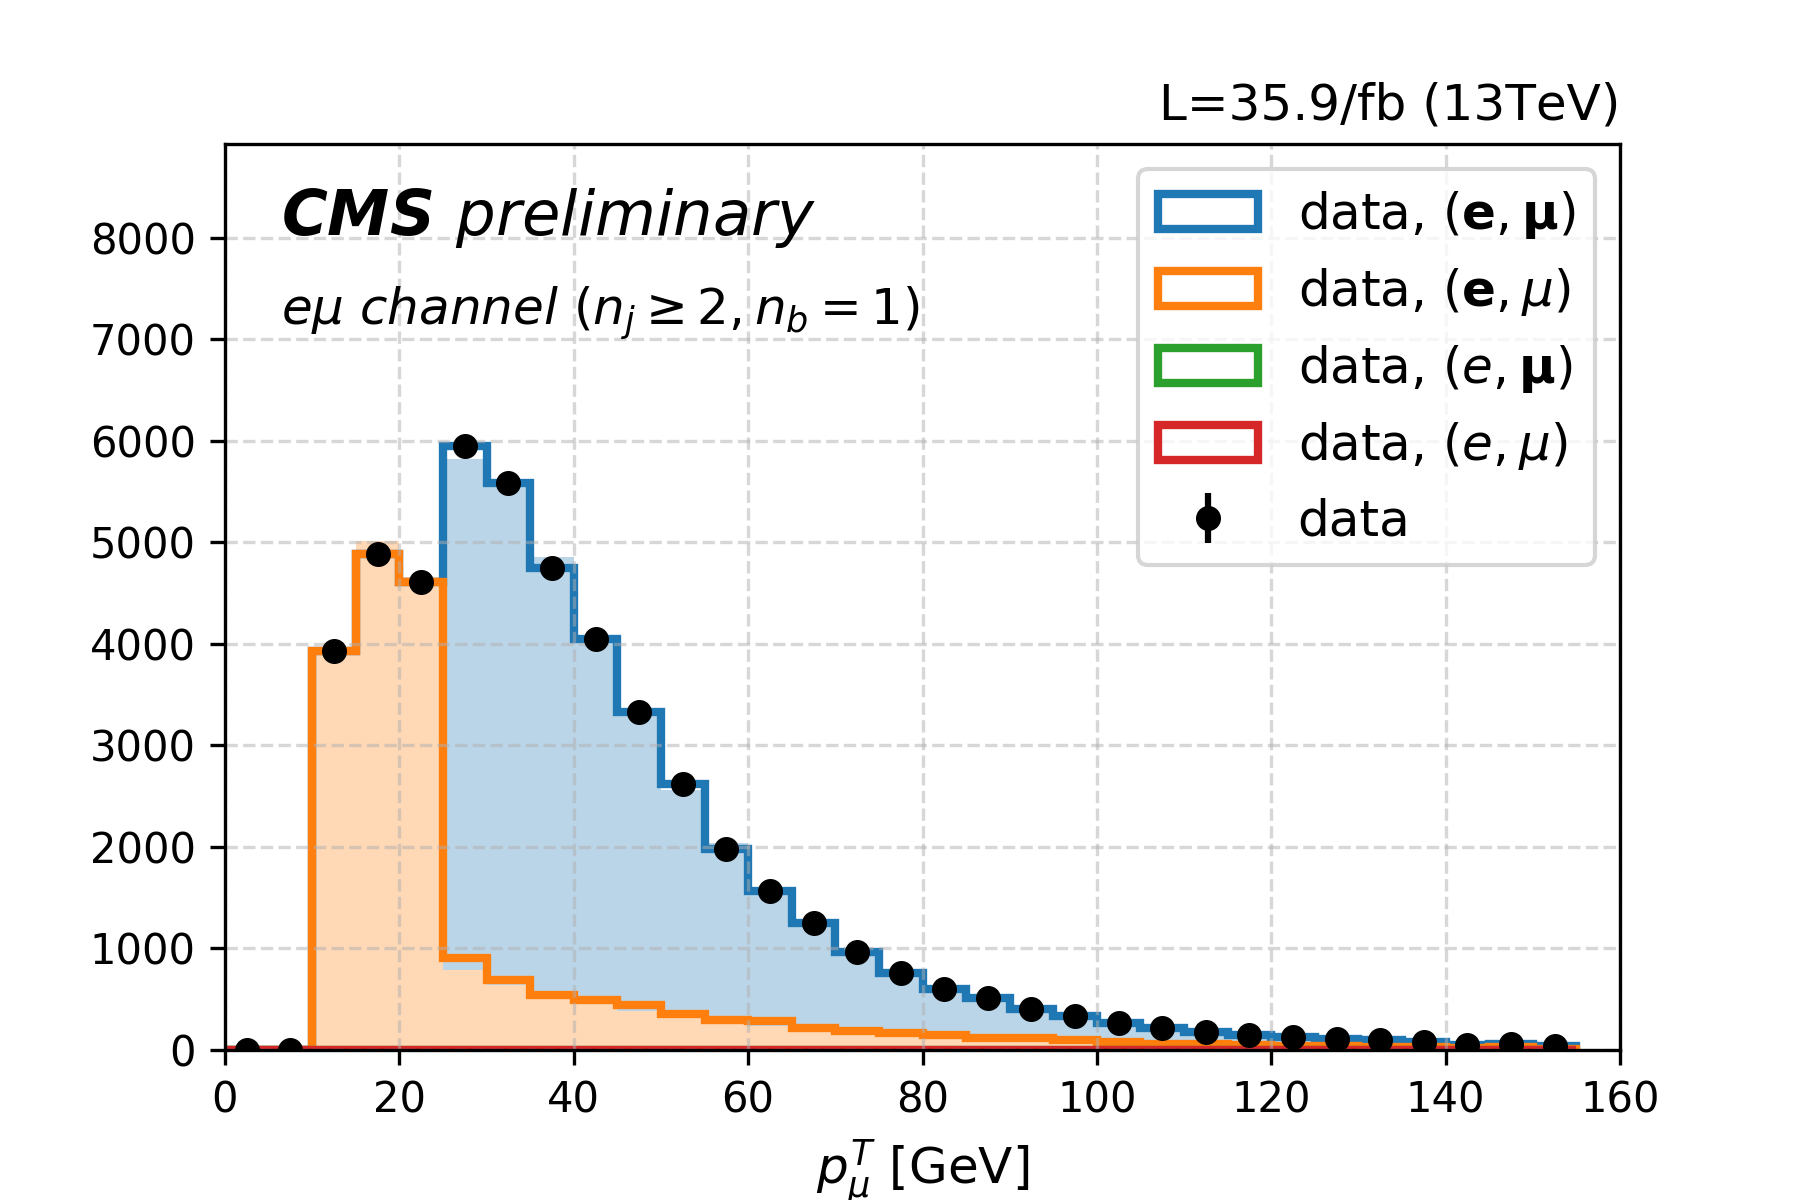
\includegraphics[width=0.49\textwidth]{chapters/Appendix/sectionTriggerTest/figures/trgLep_emu2.png}
  \caption{trailing lepton \pt in the $\mu\mu$,$ee$,$\mu e$,$e\mu$ channel. Data and MC events channel are split 
  based on the trigger test of leading and trailing lepton.
  \label{fig:triggerTest}}
\end{figure}
\FloatBarrier
